\documentclass{article}


\usepackage{hyperref}
\hypersetup{colorlinks, %
	citecolor=black,%
	filecolor=black,%
	linkcolor=black,%
	urlcolor=black,%
	pdftex}	
\usepackage{graphicx}
\usepackage{tikz}
\newcommand{\email}[1]{\texttt{#1}}
\newcommand{\st}{Conors$^{3}$}
\newcommand{\vim}{\href{http://www.vim.org} {www.vim.org} }

\title{\st{} Maths Grinds}
\author{Conor Gilmer $<$\href{mailto:conor.gilmer@gmail.com}{conor.gilmer@gmail.com}$>$}


\begin{document}
\pagestyle{headings}
\maketitle

\tableofcontents


\newpage
\section{The Prologue}
I\footnote{\email{ \href{mailto:conor.gilmer@gmail.com.com}{conor.gilmer@gmail.com} }} am just going to outline the rules and formulae which are needed for the GMAT Mathematics test.

\newpage
\section{Topics}

The topics covered

\begin{itemize}
\item Geometry
\item Algebra
\item Aritmetic
\item Problem Solving
\end{itemize}


\newpage
\section{Prerequistes and Definitions}
\begin{itemize}
\item \textbf{Natural Number} - a number which occurs in nature, an integer, a positive whole number e.g. 1,2,3,4,511 etc.,
\item \textbf{Real Number} - any number which can be plotted on a line e.g $3, 2/3, -0.2, \sqrt{3}$
\item \textbf{Imaginary Number} - a number which can not be calculated e.g. $\sqrt{-5}$
\item \textbf{Rational Number} - a number which can be written as a fraction e.g. $4 (4/1) , 2/3$
\item \textbf{Irrational Number} - a number which can not be written as a fraction e.g $\sqrt{2}, \pi, 0.271271271271...$
\end{itemize}

\textbf{Multiplying}

$+a * +b = +ab$

$+a * -b = -ab$

$-a * +b = -ab$

$-a * -b = +ab$


\textbf{Indices}

$a^{2} * a^{3} = a^{2+3} = a^{5}$

$a^{3} / a^{2} = a^{3-2} = a^{1} = a$

$a^{2} / a^{3} = a^{2-3} = a^{-1} = 1/a$

$ 0^{x} = 0 \quad \textrm{e.g.} \quad  0^{1} = 0$

$ x^{0} = 1 \quad \textrm{e.g.} \quad  x^{0 =1}$

\textbf{Ratio} - the Ratio of A to B is written as $ A/B \ or \ A : B$

\textbf{Percentage} - to get a percentage of a fraction your multiply by 100 so $ ( 3/4 ) * 100 = 75\%$

\newpage
\section{Geometry}

\begin{itemize}
\item Lines
\item Four-sided figures
\item Triangles
\item Pythagoras
\item Circles
\item Volume and Surface Area
\item Polygons
\end{itemize}

\subsection{Lines}
A Line is said to be 180 degrees, so if you know the angle one makes intersecting a line you know the other side
\subsection{Intersecting Lines}
The opposite angles in intersecting lines are equal.
\subsection{Line intersecting Parallel Lines}
Parallel lines the angles are preserved, i.e. the angles made by the intersecting lines are the same

\newpage
\subsection{Four-sided figures}
\begin{enumerate}
\item Rectangles
\item Squares
\item Parallelograms
\item Other foursided figures
\end{enumerate}
\subsubsection{Area of a Rectangle}
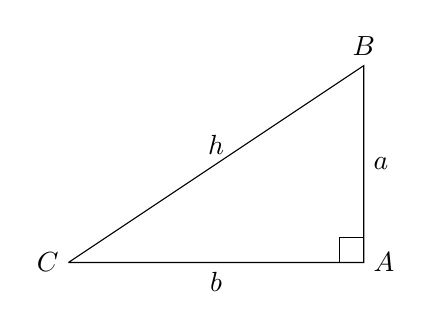
\begin{tikzpicture}[scale=1.25]%,cap=round,>=latex]

\coordinate [label=left:$C$] (A) at (-1.5cm,-1.cm);
\coordinate [label=right:$A$] (C) at (1.5cm,-1.0cm);
\coordinate [label=above:$B$] (B) at (1.5cm,1.0cm);
\draw (A) -- node[above] {$h$} (B) -- node[right] {$a$} (C) -- node[below] {$b$} (A);

\draw (1.25cm,-1.0cm) rectangle (1.5cm,-0.75cm);

\end{tikzpicture}

Area of a rectangle is the length of the sides multiplied together.
\begin{equation}
Area_{rectangle} = width * height
\end{equation}
\subsubsection{Perimeter of a Rectangle}
Is the sum of the 4 sides
\begin{equation}
Perimeter_{Rectangle} = or 2width + 2 heignt\\
or\\
Perimeter_{rectangle} = 2 ( width + height )
\end{equation}
\newpage
\subsection{Triangles}
\begin{enumerate}
\item Perimeter of a Triangle equals sum of 3 sides
\item Area of a Triangle equals half the base by perpendicular height
\item The sum of the angles of a triangle equal 180 degrees
\item Equilateral Triangle - all the angles are 60 degrees, and all sides are the same length
\item Isoceles Triangle - 2 angles are the same and 2 sides are the same length
\end{enumerate}
\subsubsection{Perimeter of a Triangle}
Perimeter of a triangle is the sum of the 3 sides so
Perimeter = Side A + Side B + Side C
\subsubsection{Area of a Triangle}
\begin{equation}
Area_{Triangle} = base * Perpindicular Height / 2
\end{equation}
\subsubsection{Angles in a Triangle}
The angles in a triangle equal 180 degrees
So if you have two angles you always can deduct the third.
\newpage
\subsection{Pythagoras Theorem}
The most important theorem In a Right angle triangle(one angle = $90^{\circ}$), the square on the hypoteneuse (longest side) is equal to the sum of the squares on the other two sides

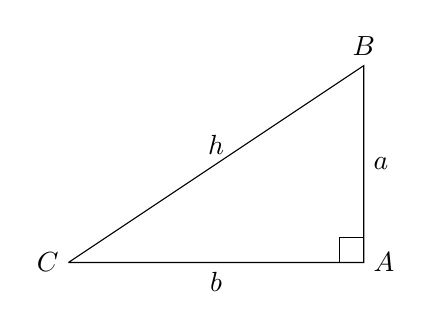
\begin{tikzpicture}[scale=1.25]%,cap=round,>=latex]

\coordinate [label=left:$C$] (A) at (-1.5cm,-1.cm);
\coordinate [label=right:$A$] (C) at (1.5cm,-1.0cm);
\coordinate [label=above:$B$] (B) at (1.5cm,1.0cm);
\draw (A) -- node[above] {$h$} (B) -- node[right] {$a$} (C) -- node[below] {$b$} (A);

\draw (1.25cm,-1.0cm) rectangle (1.5cm,-0.75cm);

\end{tikzpicture}

\begin{equation}
h^2 = a^2 + b^2
\end{equation}
so $h= \sqrt{a^2 + b^2}$
\subsubsection{Also works for the Circle on the Hypoteneuse}


\begin{equation}
\pi (h/2)^2 = \pi (a/2)^2 + \pi(b/2)^2
\end{equation}

You will find that often the numbers used in examples are triangles with sides 5, 4 and 3, 10, 8 and 6 or 50, 40 and 30 which all neatly square etc.

\newpage
\subsection{Circles}
\subsubsection{Area of a Circle}
\begin{equation}
Area = \pi r^ 2
\end{equation}
\subsubsection{Circumference of a Circle}
\begin{equation}
Area = 2 \pi r
\end{equation}
\subsection{Sectors of a Circle}
A sector of a Circle of 
\subsubsection{Area of a Sector of a Circle}
\begin{equation}
Area = ( angle / 360 ) \pi r^ 2
\end{equation}


\subsubsection{Circumference of a Sector of a Circle}
\begin{equation}
Area = ( angle / 360 ) 2 \pi r
\end{equation}

\newpage
\subsection{Volume and Surface Area}
\subsubsection{Rectangular Box}
\begin{itemize}
\item Volume of a Rectangular Box - Length by Breath by Height
\item Surface Area, is six rectangle, two breath by depth plus two breath by height plus two height by depth
\end{itemize}

\begin{equation}
Volume = width * height * depth
\end{equation}

\begin{equation}
Surface_Area = 2(width * height) + 2(width * depth) + 2(height * depth)
\end{equation}

\subsubsection{Cylinder}
\begin{itemize}
\item Volume of a Cylinder is area of the base by the height
\item Surface area is 2 circles and a rectangle (from the rolled out tube of the cylinder) height by circumference of the circle
\end{itemize}

\begin{equation}
Volume_{ Cylinder} = h \pi r^ 2
\end{equation}


\begin{equation}
Surface Area_{ Cylinder} = 2 \pi r h + 2(\pi r^ 2 )
\end{equation}

\newpage
\subsection{Polygons}
\subsubsection{Area of a Polygon}
To get a polygons area, you break it up into triangles or triangles and rectangles, may need pythagoras.
\subsubsection{Perimeter of a Polygon}
The sum of the lengths of its sides
\subsubsection{Sum of angles of a polygon}
Sum of the triangles which meet the points of the polygon - i.e. multiples of 180
Or triangle is 180, rectangle 360, adding another side will always be adding another triangle so
pentagon is 540, hexagon is 720 and heptagon is 900 and octagon 1060 and so on...

\newpage
\subsection{Slope of a Line}
There are two ways which get you the slope of a line one is with the co-ordinates the other with an equation which you resolve to look like y = mx + b where m is the slope of the line

\textbf{Using the Equation}

\begin{equation}
y = mx + B
\end{equation}

\textbf{Using Co-ordinates}

With co-ordinates ($x_1$, $y_1$) and ($x_2$, $y_2$) 
\begin{equation}
m = (y_2 - y_1) / (x_2 - y_1) 
\end{equation}


\newpage
\section{Algebra}
\subsection{Solve an Equation one Variable}
In this case you just manipulate the equation so as the variable is on one side on its own and what it equals is on ther other

\begin{equation}
2x - 9 = 1 \
2x = 1 + 9\ 
2x = 10\
x = 10 /2 
x = 5
\end{equation}

\newpage
\section{Colophon}

Wouldn't have been possible without Mr Euclid and Mr Pythagoras.

This document was written created using \LaTeX{}. 

Initially it was word-processed using text editor \href{http://www.vim.org}{www.vim.org} and then rendered into pdf using pdfplatex. 

The amendments from the original version were made using Version 2.4 of MiKTeX(\href{http://www.miktex.org}{www.miktex.org})
However since using the macbook a lot of late I use \TeX{} Live ( \href{https://www.tug.org/texlive/}{www.tug.org/texlive/}).


%It was tested using the Adobe $^{\textregistered}$ Reader 7.0 (Version 7.0.3).



\copyright 2015 Conor Gilmer $<$\href{mailto:conor.gilmer@gmail.com}{conor.gilmer@gmail.com}$>$ all rights reserved.

\end{document}

